
\subsubsection{Data re-uploading for a universal quantum classifier}
\textbf{Background}

% Run-Hong He, State Key Laboratory of Computer Science, Institute of Software Chinese Academy of Science, BeiJing 101408, China

Data classification is not only an important application of classical neural networks but also of quantum information and quantum computation in the future. Generally speaking, the structure of a quantum classifier can be divided into three main components: the sub-circuit responsible for encoding data, the sub-circuit used for information processing, and the measurements applied for extracting classification result from the final state. 
The key to achieving accurate data classification lies in capturing the nonlinear features of the data. Many approaches carefully design quantum circuits to introduce this capability, such as the strategies inspired in artificial neural networks or kernel methods that widely used in classical machine learning \cite{PhysRevLett.122.040504, 2019Supervised_nature, Wan_2017_npjqi, hur2022quantum, chalumuri2021hybrid, oh2020tutorial, farhi2018classification, wrobel2021application}. Among them, the schemes that require fewer resources such as the number of qubits and quantum operations have received widespread attention during the current NISQ devices era.
Therefore, a natural motivation is to explore the minimum resources required to construct an effective quantum classifier.

It has been shown in Ref.~\cite{PerezSalinas2020datareuploading} that a single qubit, with the assistance of a classical subroutine, can provide sufficient computational capabilities to perform multi-classification tasks for multi-dimensional input data, similar to a single hidden-layered neural network. This may sound surprising, especially considering that a single qubit provides only a superposition of two sample states and operations on it merely involve rotations around the Bloch sphere. 
The pivotal point of this scheme is to combine the data uploading unit and information processing unit and repeat them many times, i.e., \textit{Data re-uploading} to introduce the non-linearity necessary for a supervised classification task. 

The authors proved in their work that the equivalence between the data re-uploading scheme and the well-known Universal Approximation Theorem \cite{HORNIK1991251}, which argues that a single-layer network composed of enough neurons along with an activation unit can approximate any continuous function.

\begin{figure}[H]
\centering
\subfigure[ ]{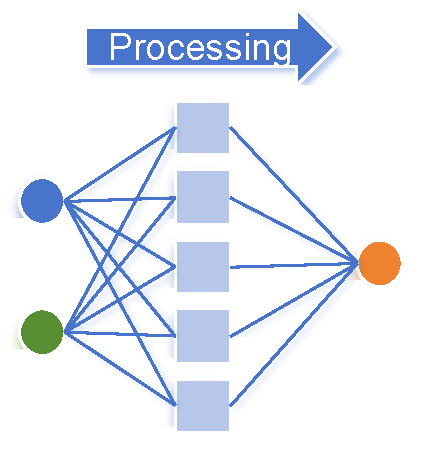
\includegraphics[width=0.18\textwidth]{5.4.3_figures/data_reuploading_neural_network.pdf}}
\subfigure[ ]{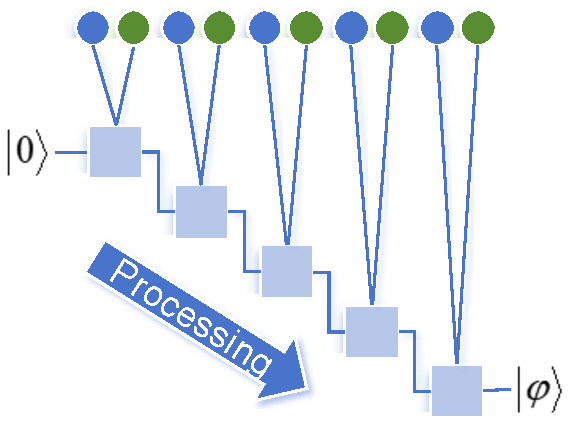
\includegraphics[width=0.24\textwidth]{5.4.3_figures/data_reuploading_quantum_classifier.pdf}}
\caption{Simplified workflows of (a) a single-hidden-layered classical neural network and (b) a single-qubit quantum classifier with structure of data re-uploading.
In the classical neural network, each neuron receives all input data. Conversely, the qubit receives both the input data and the result of previous operations.  It processes the combined information, and the final output is a quantum state that encodes multiple repetitions of input uploads and processing parameters.}
\label{diagram_data_reuploading}
\end{figure}

We precede the construction of the single-qubit classifier with an insight into the workflow of a classical single-layer neural network.
As it is shown in Fig~\ref{diagram_data_reuploading} (a), the  original data is fed into and processed by each neuron, or in other words, the original data is re-uploaded multiple times. And then in conjunction with the activation function, this feed-forward neural network captures nonlinearity.

In order to introduce this capacity to the single-qubit classifier, we have also to re-upload the data into the qubit repeatedly, and without violating the principle of quantum no-cloning theorem. The data re-uploading scheme \cite{PerezSalinas2020datareuploading} is specifically designed to address this problem, and its workflow is depicted in Fig~\ref{diagram_data_reuploading} (b). In a similar manner to the classical neural network, data points are introduced simultaneously into each processing unit, represented by a unitary rotation, of single-qubit quantum classifier. 
However, the processing units are not only affected by the input data but also by the previous processing units.
The resulting output is a quantum state that will be measured to extract the classification result.

\begin{figure}[H]
\centering
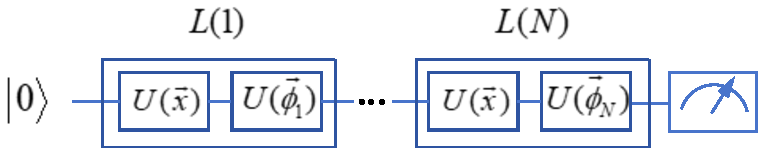
\includegraphics[width=0.45\textwidth]
{5.4.3_figures/data_reuploading_circuit.pdf}
\caption{The single-qubit classifier with data re-uploading is comprised of layers $L(i)$, which serve as the building blocks of the quantum circuit. Each of these layers consists of a $U(\overrightarrow{x})$ gate, responsible for data uploading, and a trainable parameterized unitary $U(\overrightarrow{\phi})$. We repeat this building block $N$ times and calculate a cost function, which is related to the fidelity between the final state of the circuit and the corresponding target state of its class.}
\label{data_reuploading_circuit}
\end{figure}

The explicit form of this single-qubit classifier is
shown in Fig~\ref{data_reuploading_circuit}. Classical data is repeatedly re-uploaded in a sequential manner, with processing units interspersed between them. The introduced data can be represented as qubit rotations.  A data point from 3-dimentsional space, $\overrightarrow{x}$, can be re-uploaded by a rotation of the qubit $U(\overrightarrow{x})$. Subsequent processing units are also rotations, whose angles will be optimized as trainable parameters to minimize the cost value $C(F)$ for performance improvement. The fidelity $F$ quantifies the closeness between the final state of the circuit and the target state corresponding to the label.

Then, the overall function of this quantum circuit is 
$$\mathcal{U}(\overrightarrow{\phi},\overrightarrow{x})=U(\overrightarrow{\phi}_N)U(\overrightarrow{x})\cdots U(\overrightarrow{\phi}_1)U(\overrightarrow{x}),$$
which acts as 
$$|\varphi\rangle=\mathcal{U}(\overrightarrow{\phi},\overrightarrow{x})|0\rangle.$$
The final classification of the data point will be determined by the measurement result on $|\phi\rangle$. Each pair of data uploading unit and processing unit can form a processing layer together:
$$L(i)\equiv U(\overrightarrow{\phi}_i)U(\overrightarrow{x}),$$
thus the classifier corresponds to 
$$\mathcal{U}(\overrightarrow{\phi},\overrightarrow{x})=L(N)\cdots L(1).$$

The authors note that increasing the number of layers can provide the circuit with stronger expressivity, and leading to a higher classification accuracy.

\textbf{\textit{Target Problem:}}

Constructing and training a single-qubit data re-uploading quantum circuit to classify classical data.

\textbf{\textit{Required MindSpore Quantum functionalities:}}

1. Allowing the construction of interleaved and repetitive encoder and ansatz circuits, as well as enabling data re-uploading to the encoders.

2. Batching training over input data (multiple data and labels).

\textbf{Implementation}

In this example, we focus on a typical classification task: identifying points in different areas of a plane, and implement it based on MindSpore Quantum.
The full notebook and implementation for this example is avaliable at: XXXXXXXXX.

We create a dataset comprising numerous points with coordinates $\overrightarrow{x}=(x_1, x_2)$  randomly distributed on a unit area plane ($x\in[-1,1]$). 
The task of the classifier is to determine, based on the coordinates of these data points, whether they fall within a circle of radius $r$, i.e., $x_1^2+x_2^2<r^2$.
And the radius of the circle is intentionally set to $r=\sqrt{\frac{2}{\pi}}$ to ensure an equal probability of points being inside (labeled `0' and corresponding to the target quantum state $|0\rangle$) or outside (labeled `1' and corresponding to the target quantum state $|1\rangle$) the circle.

\begin{lstlisting}
import numpy as np  

def data_gen(n_samples=1000):
    center=[0.0, 0.0]
    rad=np.sqrt(2/np.pi)
    data, labels = [], []
    for i in range(n_samples):
        x = 2*(np.random.rand(2))-1
        if np.linalg.norm(x-center) <= rad:
            y = 0
        else:
            y = 1     
        data.append(x)
        labels.append(y)
    return np.array(data), np.array(labels)
        
train_data, train_labels = data_gen(1000)
eval_data, eval_labels = data_gen(500)
test_data, test_labels = data_gen(5000)
\end{lstlisting}

The training set, validation set, and test set we created consist of 1000, 500, and 5000 random samples, respectively.

To encode the data onto the qubit, we use angles of rotation around the $x$ and $z$ axes to represent the coordinate information of the samples, i.e. $U(\overrightarrow{x})=U(x_1,x_2,0)=RZ(x_2)RX(x_1)$.  Since our samples to be classified are only 2-dimensional, here we have padded 0.
Input data ($[x_1, x_2, x_3, \cdots x_{N-2}, x_{N-1},x_{N}]$) with $N$ dimensions can be split into multiple sets of three-dimensional components for encoding $U(\overrightarrow{x})=U(x_{N-2},x_{N-1},x_{N})\cdots U(x_1,x_2,x_3)$.

Next, we construct the circuit for a single-qubit classifier. We begin by applying a $H$ gate to the initial quantum state to generate a superposition state $(|0\rangle+|1\rangle)/\sqrt{2}$.
Afterwards, we add $RZ(x_1)$ and $RX(x_2)$ gates to upload the sample's  coordinates $x_1$ and $x_2$ onto the qubit. 
The subsequent processing unit is represented by a $U3$ gate with three independent trainable parameters to act as an arbitrary rotation.
These two sub-circuits are also named as ``encoder" and ``ansatz" respectively to indicate the parameters of the rotation gates will be directly fed into or gradually updated during training.
The encoder and ansatz together form a layer, and multiple such layers can be repeated to achieve the functionality of multiple data re-uploading and processing, thereby enabling points classification.

\begin{lstlisting} 

from mindquantum import H, RZ, RX, U3, BarrierGate, Circuit, Simulator, Hamiltonian, QubitOperator, MQLayer

def circ(depth=1):
    circ = Circuit(H.on(0))
    circ += BarrierGate()
    for layer in range(depth):
        circ += Circuit([RZ('x1').on(0), RX('x2').on(0)]).as_encoder()
        circ += Circuit(U3(f'theta_{layer}', f'phi_{layer}',f'lambda_{layer}').on(0)).as_ansatz()
        circ += BarrierGate()
    return circ

example_circ = circ(depth=1)
example_circ.svg()
\end{lstlisting}

\begin{figure}[H]
\centering
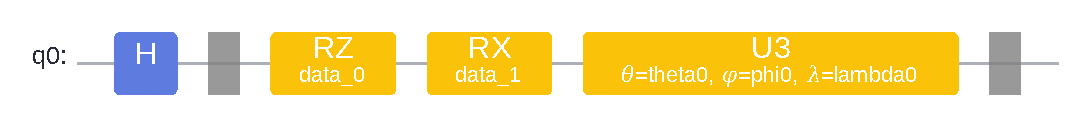
\includegraphics[width=0.49\textwidth]
{5.4.3_figures/data_reuploading_circ0.pdf}
\caption{The schematic diagram depicts a single qubit being subjected to an 
$H$ gate to generate a uniform superposition state, along with an encoding and information processing layer for handling the classification task.}
\label{data_reuploading_circ0}
\end{figure}

The overall quantum circuit will transform the quantum state from $|0\rangle$ to $\varphi$, which requires to be measured. 
As mentioned before, the classification result `0' (inside the circle) or `1' (outside the circle) can be determined according to the final measurement of the single qubit, e.g., a sampled point can be classified into `0' if the output probabilities $P(|0\rangle)>P(|1\rangle)$ and into  `1' otherwise.  
This approach can also be represented by the energy expectation of the final quantum state along the $Z$ direction , i.e., classifies the sampled point into `0’ if $E(|\varphi\rangle)>0$ and else into `1'. Hence, the loss function can be defined as $Loss=[E(|\varphi\rangle)-(1-2\cdot\mathrm{label})]^2$.

In the following code, we utilize the Adam optimizer with a learning rate of 0.1 as a classical subroutine to train the trainable parameters in the quantum circuit. The performance of classification will be enhanced  by minimizing the loss function.


\begin{lstlisting}
import mindspore as ms
from mindspore import Tensor, ops
from mindspore.nn import Adam, TrainOneStepCell, LossBase,WithLossCell
ms.set_context(mode=ms.PYNATIVE_MODE, device_target='CPU')
import copy

circ = circ(depth=4)
ham = Hamiltonian(QubitOperator('Z0'))
sim = Simulator('mqvector', 1)
grad_ops = sim.get_expectation_with_grad(ham, circ)
qnet = MQLayer(grad_ops)

class MyLoss(LossBase):
    def __init__(self, reduction='mean'):
        super(MyLoss, self).__init__(reduction)
        self.square = ops.Square()

    def construct(self, logits, label):
        out =self.square(logits - (1-2*label))
        return self.get_loss(out)
    
loss = MyLoss()
opti = Adam(qnet.trainable_params(), learning_rate=0.02)  
model = TrainOneStepCell(WithLossCell(qnet, loss), opti)

\end{lstlisting}
If the task to be solved  with this single-qubit classifier involves many classes, one possible strategy consists on comparing the probability $P(|0\rangle)$  with several thresholds. For example, for a 4-categorized task, the determination of the classification result can be based on the interval in which the probability $P(|0\rangle)$ lies: $0\leqslant\lambda_1\leqslant\lambda_2\leqslant\lambda_3\leqslant1$.

Next, we train the parameters in the ansatzs  for 5000 iterations, recording and saving the highest validation accuracy achieved along with the corresponding trainable parameters. The batch size for training is 4.

\begin{lstlisting}
def eval(ansatz_params, eval_data, eval_labels):
    res = []
    for index in range(len(eval_label)):
        sim.reset()
        sim.apply_circuit(circ, pr=dict(zip(circ.params_name, np.hstack((eval_data[index], ansatz_params)))))
        exp = sim.get_expectation(ham).real
        clas = exp <= 0
        res.append(int(clas == eval_label[index]))    
    return np.sum(res)/len(res)

acc_list = []
acc_max = 0.0

print('Training begins ...')

for i in range(2001):
    index = np.random.randint(0,len(train_data),4)
    loss = model(ms.Tensor(train_data[index]), ms.Tensor(train_labels[index]))
    acc = eval(qnet.weight.asnumpy(), eval_data, eval_labels)
    if acc > acc_max:
        acc_max = acc
        best_params = copy.deepcopy(qnet.weight.asnumpy())
    acc_list.append(acc)
    if i % 200 == 0:
        print(f'turn:{i}\t',f'\tacc_max:{acc_max}')
        
print('Training completes.\n')
print('Maximum validation accuracy in training:\n', acc_max)

test_acc = eval(best_params,test_data,test_labels)

print('Average test accuracy:\n', test_acc)
\end{lstlisting}

\begin{lstlisting}
Training begins ...
turn:0	 	  acc_max:0.55
turn:200	 	acc_max:0.566
turn:400	 	acc_max:0.622
turn:600	 	acc_max:0.622
turn:800	 	acc_max:0.7
turn:1000	 	acc_max:0.814
turn:1200	 	acc_max:0.814
turn:1400	 	acc_max:0.814
turn:1600	 	acc_max:0.814
turn:1800	 	acc_max:0.894
turn:2000	 	acc_max:0.894
Training completes.

Maximum validation accuracy in training:
0.894

Average test accuracy: 
0.8876
\end{lstlisting}

As seen in the information printed above, the model's prediction accuracy has reached $88.76\%$, meaning that the anticipated classification results are well consistent with the actual classification results.
Fig.~\ref{data_reuploading_performance} visualizes and compares the predictions before training, predictions after training, and the true classification data. 
It can be observed that, after training, this single-qubit classifier is able to effectively classify the samples.
\begin{figure}[H]
\centering
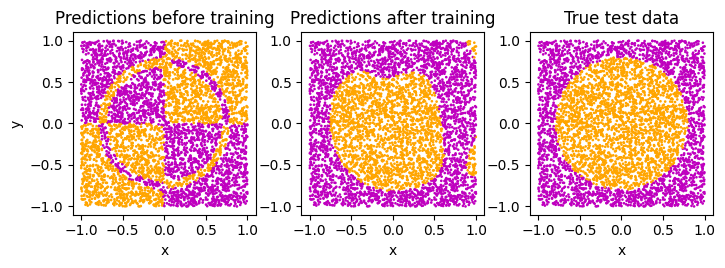
\includegraphics[width=0.49\textwidth]
{5.4.3_figures/data_reuploading_performance.png}
\caption{Visualization Comparison of the data re-uploading single-qubit classifier's predictions before training, after training, and true data.}
\label{data_reuploading_performance}
\end{figure}

In addition, the authors also extended this scheme to a multiple-qubits version and achieved further improved performance, benefiting from the resulting more complex quantum superposition states and quantum entanglement.
